\documentclass[UTF8,zihao=-4]{ctexbeamer}
\usepackage{multimedia}
\usepackage{hyperref}
\usepackage{smartdiagram}
\usepackage{listings}
\usepackage{tikz}
\usetikzlibrary{shapes.geometric,calc}
\usesmartdiagramlibrary{additions} 
\setbeamercovered{highly dynamic}

%% 所要粘贴代码的编程语言
%\lstloadlanguages{}

%% 设置listings宏包的一些全局样式
%% 参考http://hi.baidu.com/shawpinlee/blog/item/9ec431cbae28e41cbe09e6e4.html
\lstset{
	showstringspaces=false,              %% 设定是否显示代码之间的空格符号
	numbers=left,                        %% 在左边显示行号
	numberstyle=\tiny,                   %% 设定行号字体的大小
	basicstyle=\footnotesize,                    %% 设定字体大小\tiny, \small, \Large等等
	keywordstyle=\color{blue!70}, commentstyle=\color{red!50!green!50!blue!50},
	%% 关键字高亮
	frame=shadowbox,                     %% 给代码加框
	rulesepcolor=\color{red!20!green!20!blue!20},
	escapechar=`,                        %% 中文逃逸字符,用于中英混排
	xleftmargin=2em,xrightmargin=2em, aboveskip=1em,
	breaklines,                          %% 这条命令可以让LaTeX自动将长的代码行换行排版
	extendedchars=false                  %% 这一条命令可以解决代码跨页时,章节标题,页眉等汉字不显示的问题
}

\usetheme{Madrid}
%\useoutertheme{miniframes}

\usecolortheme{orchid}
\title{孔加工概述~~说课}
\author{高星}
\institute{湖南潇湘技师学院~湖南九嶷职院}
\date{2017.12.1\\[0pt]}
\begin{document}
    
\begin{frame}[plain]
	\maketitle
	\noindent
	
	\centering	\begin{tabular}[t]{*{4}{l@{~ }}}
			\includegraphics[width=0.22\linewidth,trim=0 0 0 0,clip,angle=0]{image/1.jpg} & 
			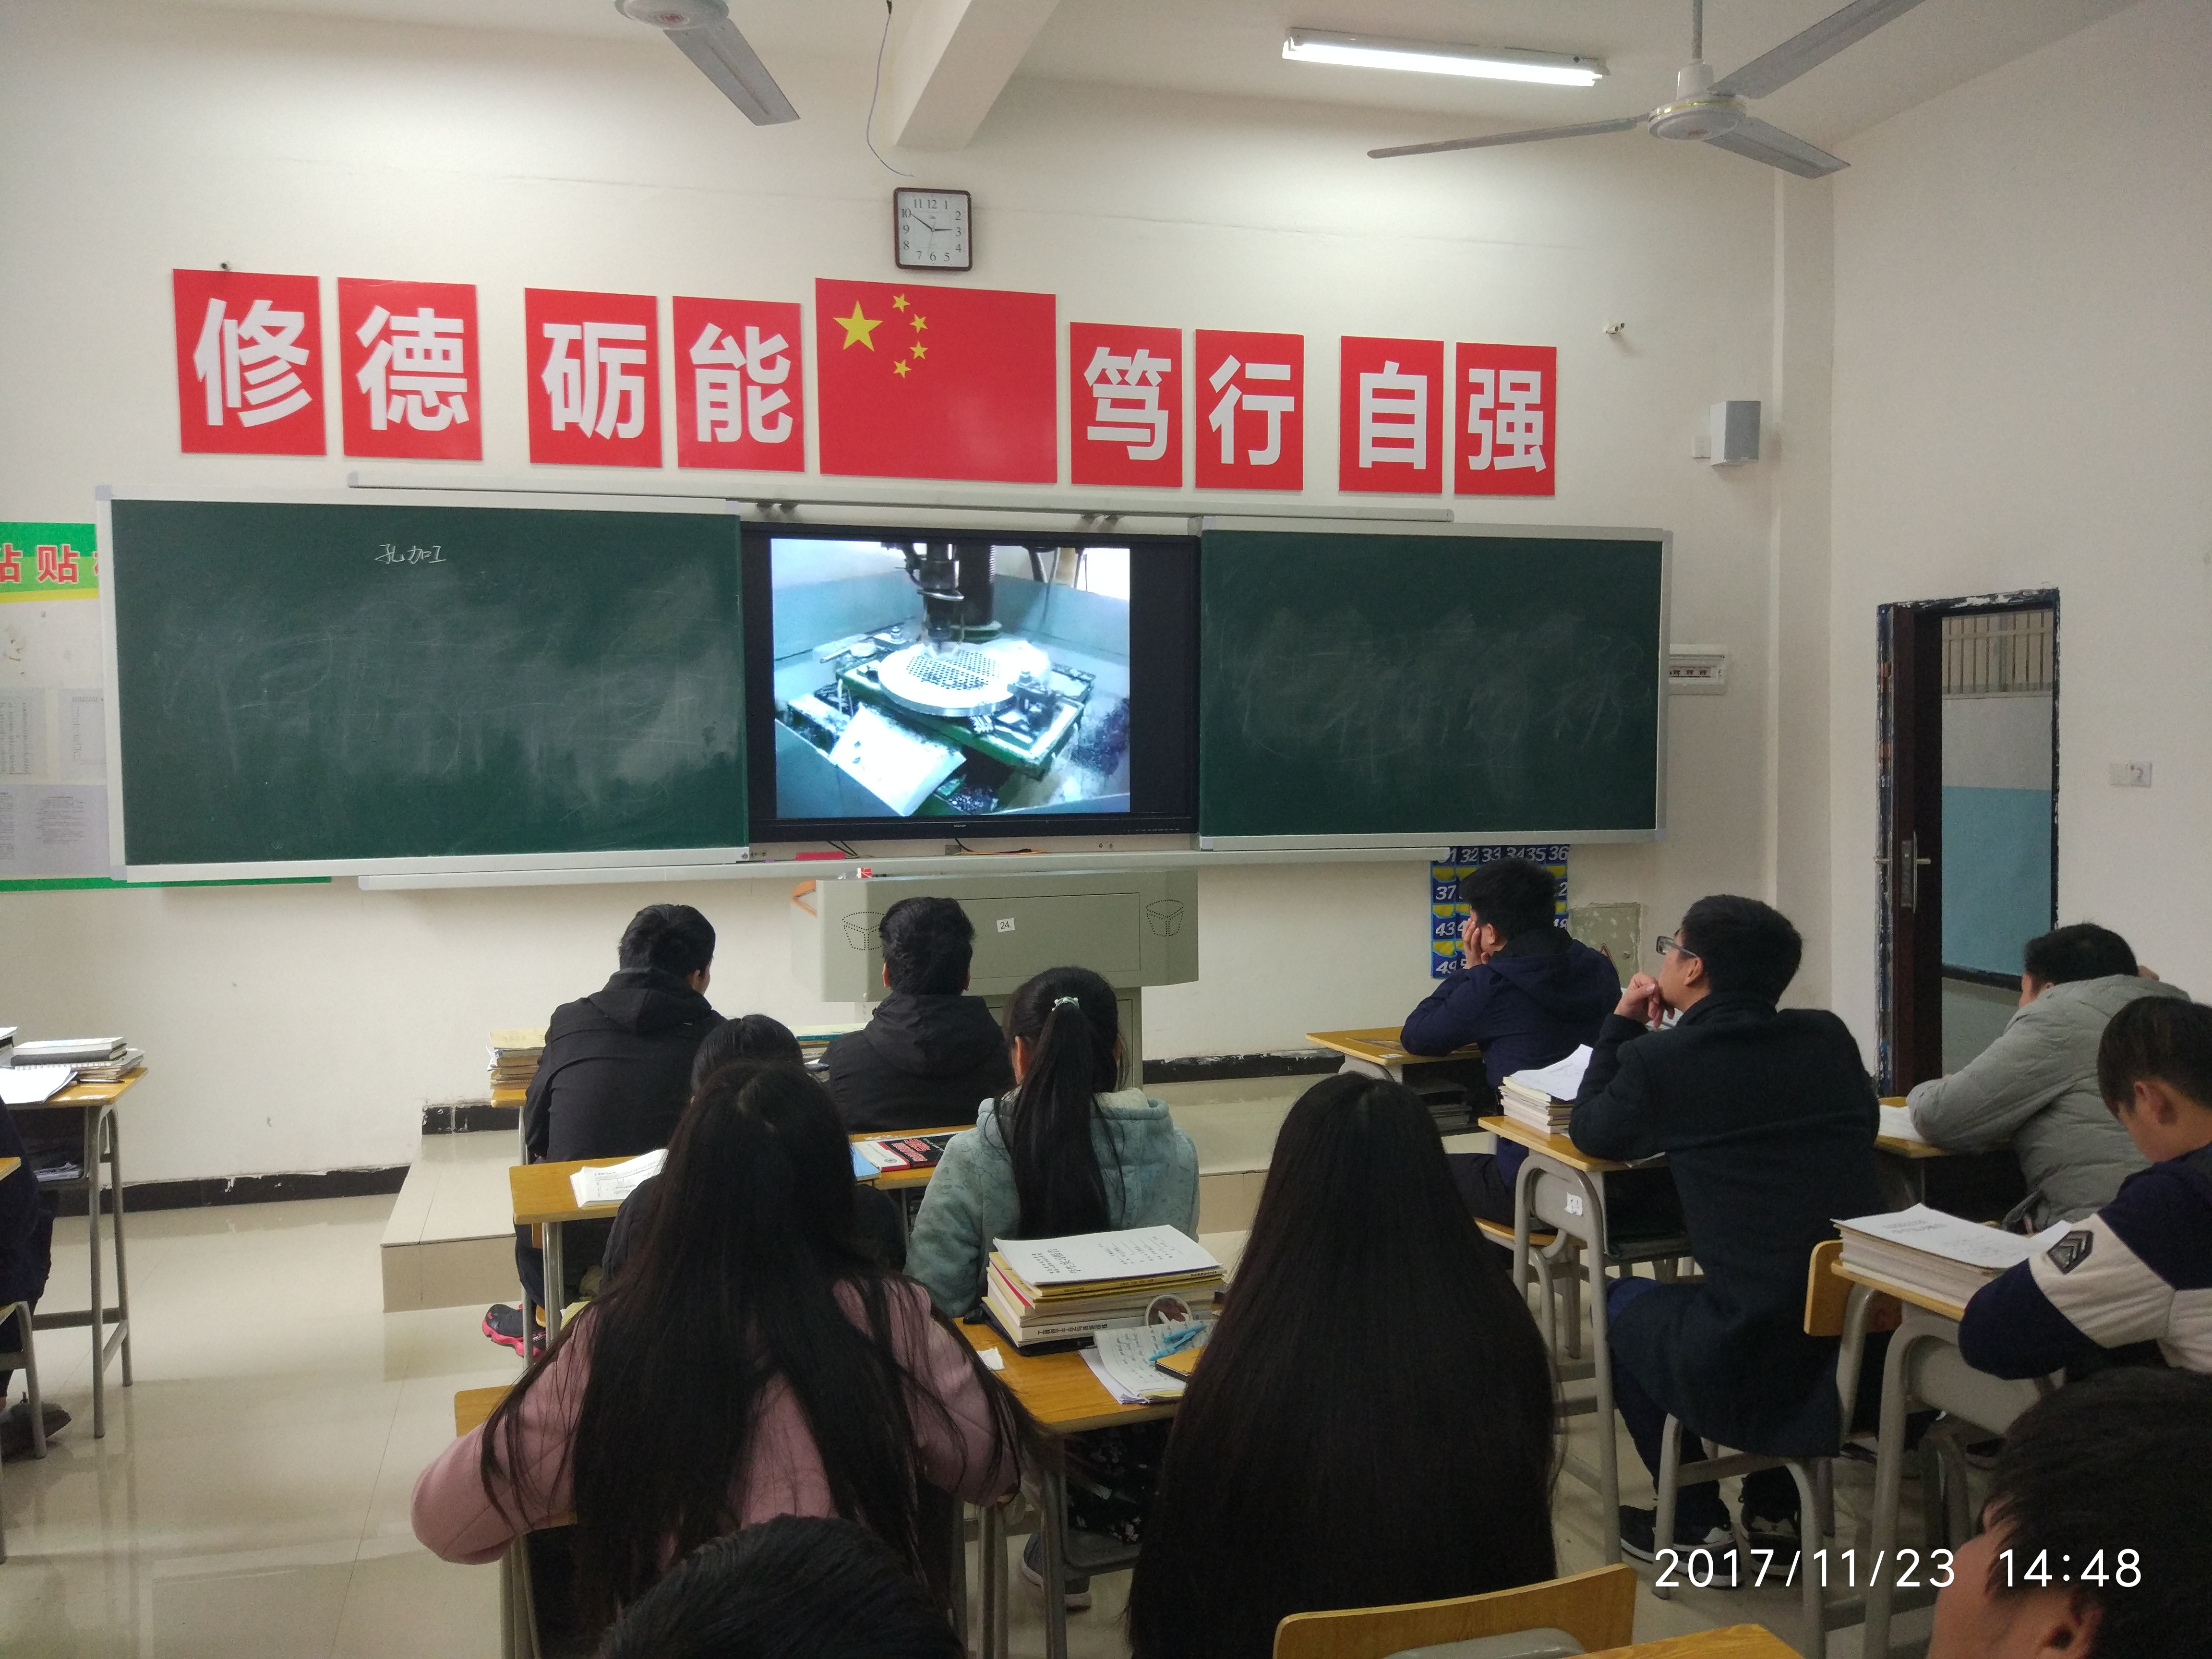
\includegraphics[width=0.22\linewidth,trim=300 0 0 12cm,clip,angle=0]{image/2.jpg}&
			\includegraphics[width=0.22\linewidth,trim=10cm 0 0 0,clip,angle=0]{image/3.jpg}&
			\includegraphics[width=0.22\linewidth,trim=10cm 0  0 0,clip,angle=0]{image/4.jpg}
	\end{tabular}
\vfill 

\end{frame}

\begin{frame}{说课内容}
\begin{columns}[onlytextwidth]

\column[c]{0.1\textwidth}
	
\column[c]{0.3\textwidth}
\tableofcontents[hideallsubsections]

\column[c]{0.6\textwidth}
\vspace{0.5cm}

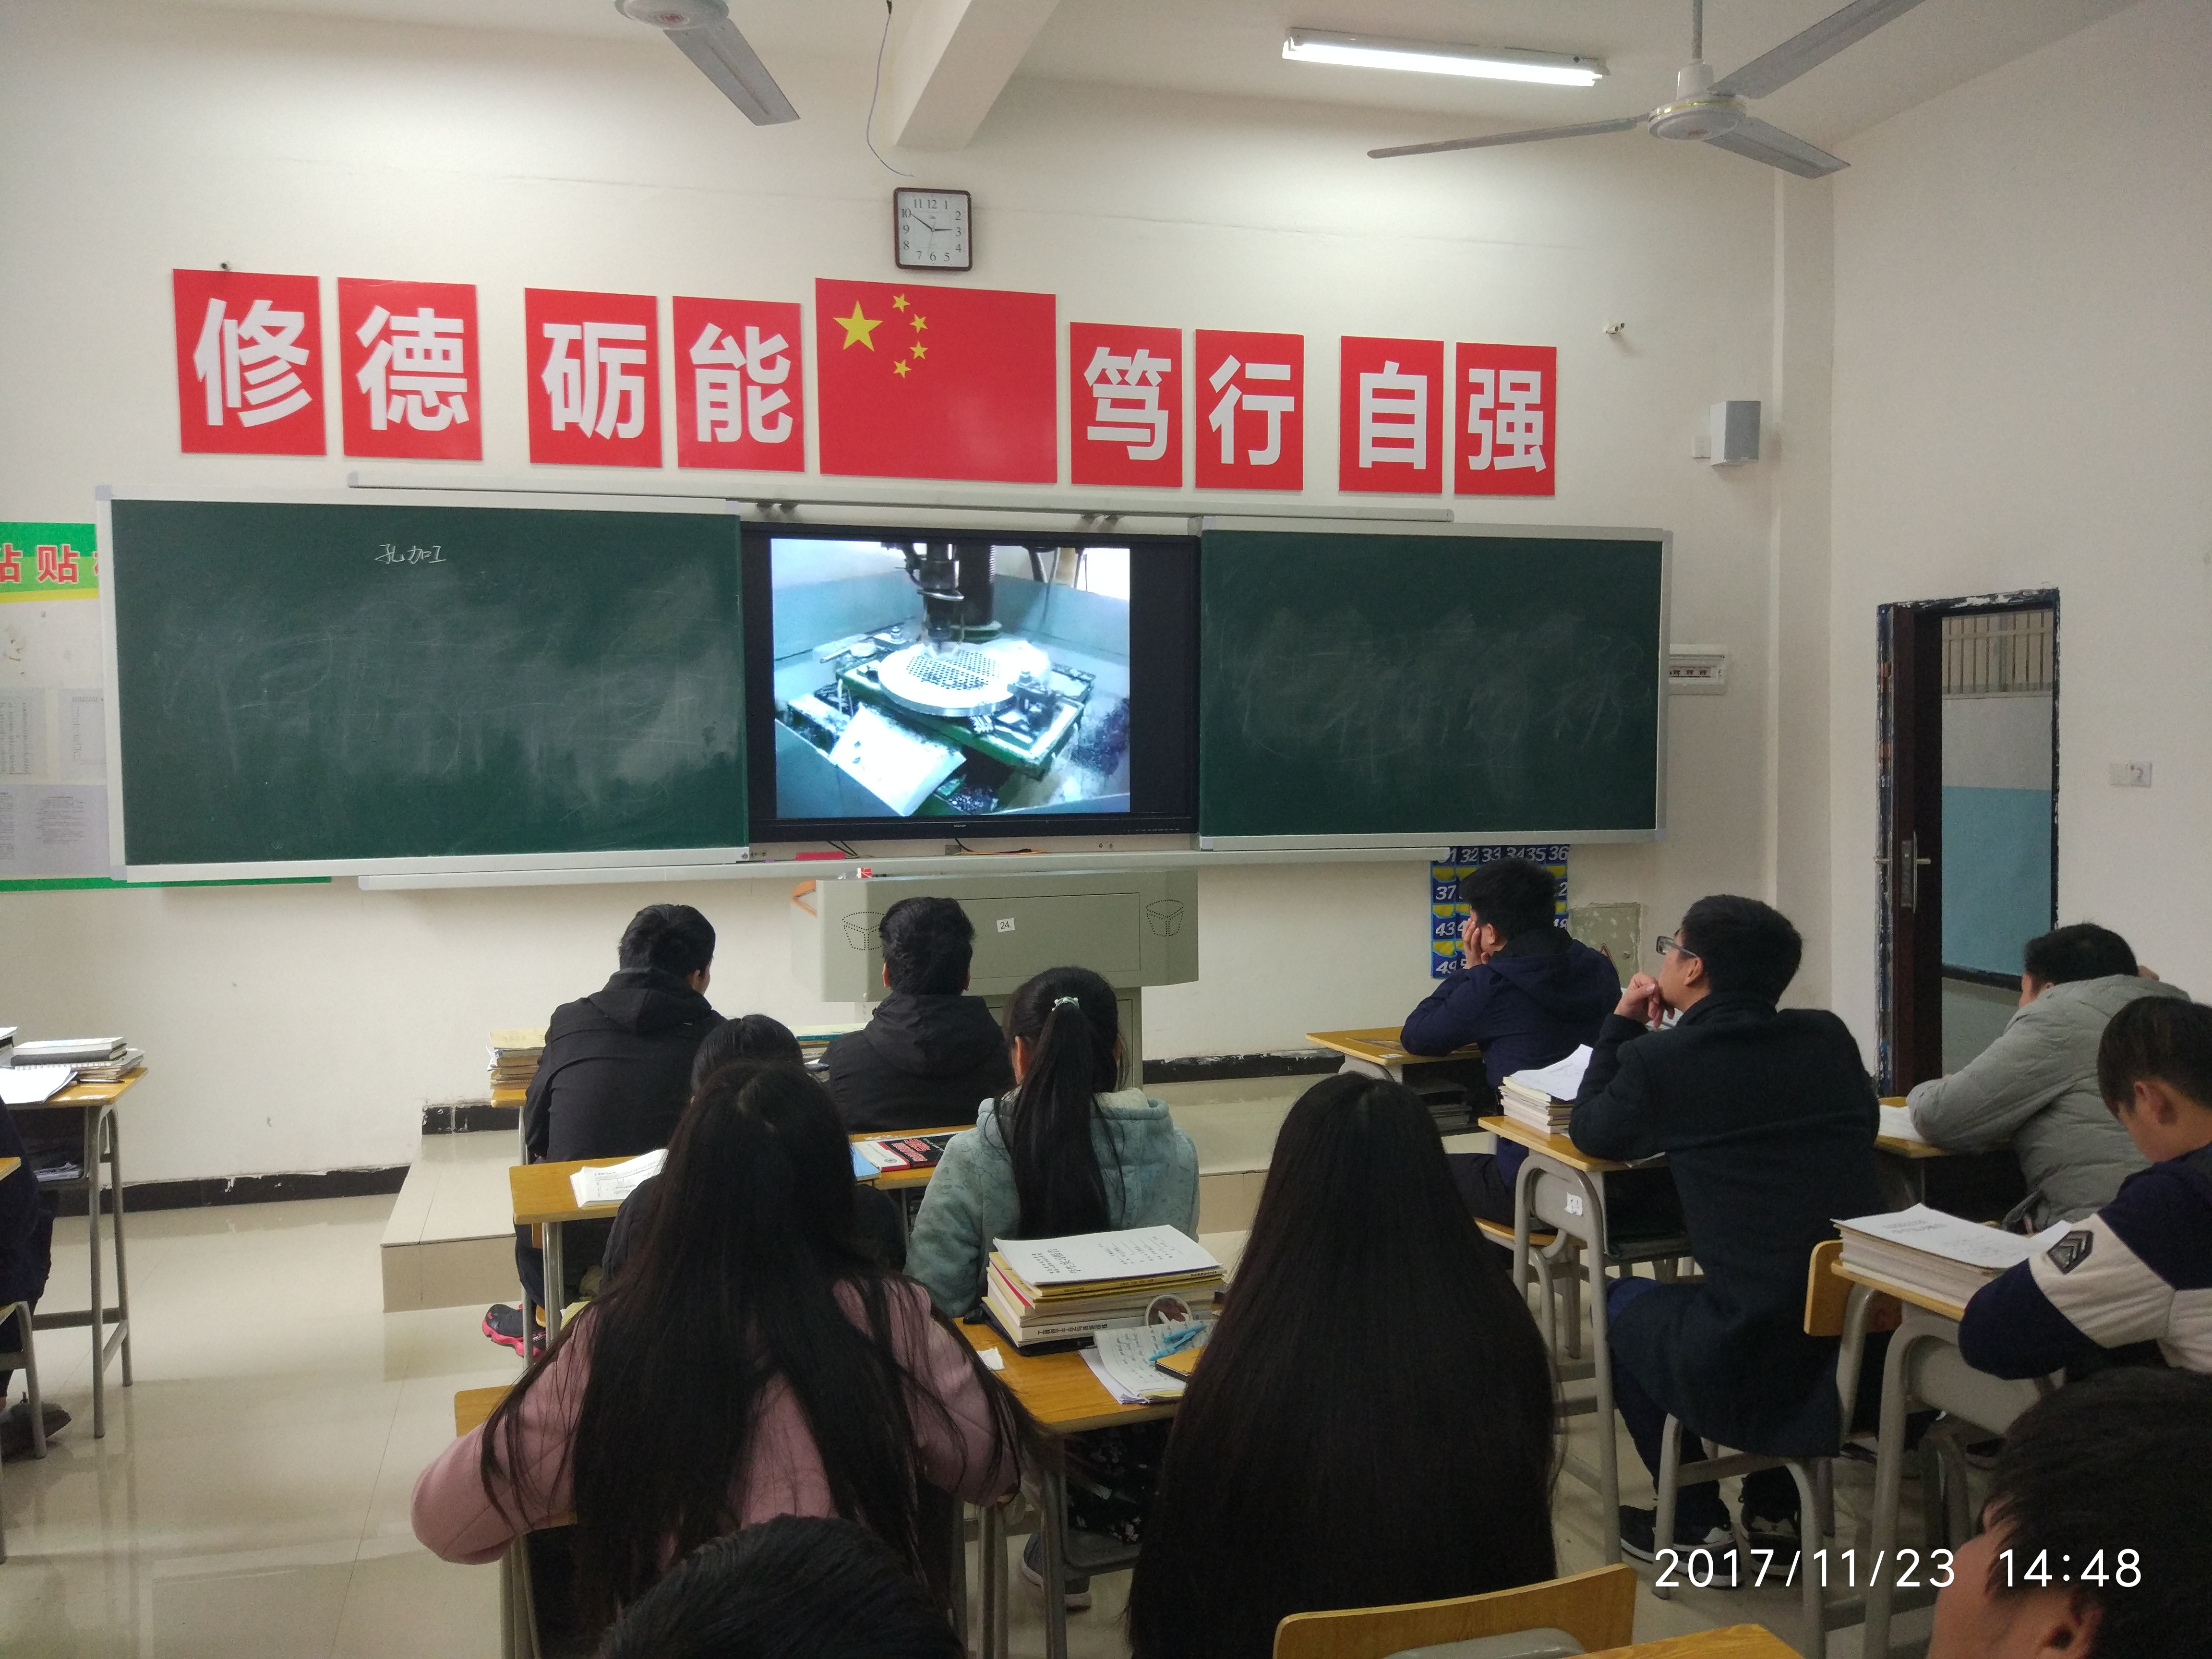
\includegraphics[width=0.9\linewidth,trim=300 0 0 12cm,clip,angle=0]{image/2.jpg}
\end{columns}

\end{frame}

\section{说教材}
\subsection{教材选择}
\begin{frame}{教材选择}
	\begin{columns}[onlytextwidth]
		\column{.2\textwidth}
		\column{.8\textwidth}
		\begin{enumerate}
			\item 掌握G1与G0的区别。
			\item 掌握G2/G3的基本应用。
			\item 能编写圆弧凸台的程序;
			\item 掌握编程基本思路。
		\end{enumerate}
	\end{columns}
\end{frame}

\subsection{教材处理}

\subsection{教学目标}

\subsection{重点难点}

\begin{frame}{重点难点}

\begin{center}
		\smartdiagramset{border color=none,
		set color list={blue!50!cyan,green!60!lime,orange!50!red,red!80!black},
		back arrow disabled=true}
	\smartdiagram[flow diagram:horizontal]{扽森扽扽三扽扽 up,扽扽我,34东方,扽三的发}
\end{center}

\end{frame}

\begin{frame}
	
	\begin{center}

\smartdiagram[priority descriptive diagram]{
	Develop a document structure,
	Choose a document class,
	Select suitable packages,dsaf撒东方东方}

	\end{center}
	
\end{frame}

\begin{frame}{重点难点}
	
	\begin{center}
		
\smartdiagram[circular diagram:clockwise]{Edit,
	pdf\LaTeX, Bib\TeX/ biber, make\-index, pdf\LaTeX,狂风e死}
		
	\end{center}
	
\end{frame}


\begin{frame}

\begin{center}
	\smartdiagram[descriptive diagram]{
	{Style,{Define shapes, colors, shading,
			and line styles for nodes and arrows}},
	{Position, {Place nodes using a matrix,
			relative or absolute positioning}},
	{Relation, Insert edges or arrows
		between selected nodes},
	{Label, Add labels on edges or arrows}}
\end{center}

\end{frame}


\begin{frame}
	
\begin{center}
\smartdiagram[bubble diagram]{\TeX\ engines,
	\TeX\ (dvi), pdf\TeX, rt, rtrt, Con\TeX t}
\end{center}
	
\end{frame}


\begin{frame}
\begin{center}
	\smartdiagram[constellation diagram]{\TeX\ software,
	Editor, Compiler, Converter, PDF Reader}
\end{center}
\end{frame}


\begin{frame}
	\begin{center}
		\smartdiagram[flow diagram:horizontal]{Edit,
			\LaTeX, Bib\TeX/ biber, make\-index, \LaTeX}
	\end{center}
\end{frame}


\begin{frame}
	\begin{center}
\tikzset{
	planet/.append style={regular polygon, regular polygon sides=6},
	satellite/.append style={regular polygon, regular polygon sides=6},
	every picture/.append style={rotate=30},
	connection planet satellite/.style={
		bend right/.style=,
		every edge/.style={fill=\col},
		to path={
			\pgfextra
			\path[draw=none, fill=none] (\tikztostart) 
			-- coordinate[at start] (@start@) coordinate[at end] (@target@) (\tikztotarget);
			\endpgfextra
			\ifnum\xi<\maxsmitem % to disable the last arrow
			($(@start@)!.6cm!90:(@target@)$) -- ($(@target@)!.25cm!-90:(@start@)$)
			-- ($(@target@)!.25cm!90:(@start@)$) -- ($(@start@)!.6cm!-90:(@target@)$)
			-- cycle
			\fi}}}
\smartdiagram[connected constellation diagram]{
	Build a program,
	Set up,
	Run,
	Analyze,
	Modify/\\Add,
	Check,
	and a sixth}
	\end{center}
\end{frame}

\begin{frame}
\begin{center}
	\smartdiagramset{
	set color list={red!10, red!30,red!50},
	sequence item border color=black,
	sequence item text color=black,
	sequence item border size=1.2\pgflinewidth,
	sequence item font size=\scriptsize\sffamily,
	additions={
		additional item shape=rectangle,
		additional item fill color=gray!20,
		additional item border color=black,
		additional arrow line width=2pt,
		additional arrow tip=to,
		additional arrow color=black,
		additional item font=\scriptsize\sffamily,
	}
}
\smartdiagramadd[sequence diagram]{step 1,step 2, step 3}
{above of sequence-item1/input,below of sequence-item2/output 1,below of sequence-item3/output 2}
\smartdiagramconnect{to-}{sequence-item1/additional-module1}
\smartdiagramconnect{-to}{sequence-item2/additional-module2}
\smartdiagramconnect{-to}{sequence-item3/additional-module3}
\end{center}

\end{frame}

%\begin{frame}
%\begin{center}
%	\smartdiagramset{diagram style, module y sep=2.5}
%	\smartdiagram[flow diagram]{Do, This,For, Me}
%\end{center}
%\end{frame}




\section{说教法}
\begin{frame}{案例分析}
     \begin{columns}[onlytextwidth]
        \column{.4\textwidth}
        在数控铣床或加工中心上加工如图所示的零件,试完成程序的编写,已知毛坯为 $\Phi$ 110*30。
        \column{.6\textwidth}

\begin{figure}
    \centering
    \includegraphics[width=0.8\linewidth,trim=50 150 50 100,clip]{image/4.jpg}
%    \caption{}
    \label{fig:4-1}
\end{figure}
    \end{columns}
\end{frame}

\begin{frame}{手工编程流程}
    \begin{columns}[onlytextwidth]
        \column{.2\textwidth}
        \column{.8\textwidth}
\begin{enumerate}
    \item 图样分析;
    \item 确定加工内容;
    \item 确定装夹及工件坐标系;
    \item 确定刀具及切削用量;
    \item 确定工序及走刀路线;
    \item 计算点坐标;
    \item 编写程序单。
\end{enumerate}
    \end{columns}
\end{frame}


\section{说学法}
\begin{frame}{G0与G1的区别}
    \begin{columns}[onlytextwidth]
        \column{.0\textwidth}
        \column{\textwidth}
\begin{enumerate}
    \item 指令格式不同:G1使用前必须用F设定进给速度,G0的速度与F无关 
    \item 运动轨迹不同:G0为快速定位,其路径可能为直线,也可能为折线。G1为直线插补,其路径为直线。
    \item 进给速度不同:G0的速度由机床参数及快速倍率决定,档位少。G1的速度由F及进给倍率决定,可调档位多。
    \item 功能用途不同:G0用于加工前的定位及加工后的提刀,G1用于车削加工
\end{enumerate}
    \end{columns}
\end{frame}


\begin{frame}{怎样确定一个圆弧}
    \begin{columns}
        \column{.3\textwidth}
        \column{\textwidth}
    \end{columns}
\end{frame}

\begin{frame}{怎样确定一个圆弧}
    \begin{columns}
        \column{.3\textwidth}
        \column{\textwidth}
        \begin{enumerate}
            \item 圆弧三点
            \item 起点、终点、圆心
            \item 2点半径
            \item 圆心、半径、起始角、终止角
            \item 其他
        \end{enumerate}
    \end{columns}
\end{frame}

\begin{frame}{数控机床圆弧编程}
    \begin{columns}
        \column{.2\textwidth}
        \column{0.6\textwidth}
        \begin{enumerate}
            \item 圆弧编程 (R)
            \item 圆心编程 (IJK)
        \end{enumerate}
         \vspace{1cm}
         圆心编程 (IJK)为标准格式,自动编程常用,手工编程一般用于整圆。
         
         圆弧编程 (R),指令符合图样标注,使用较多。
         \column{.2\textwidth}
    \end{columns}
\end{frame}

\begin{frame}{圆弧编程格式}
    \begin{columns}
        \column{0.6\textwidth}

 \begin{enumerate}
     \item XY平面的圆弧 
   
 G17  G2/G3  G90/G91 X\_ Y\_ R\_ F\_
 
 \item ZX平面的圆弧 
   
 G18 G2/G3 G90/G91 Z\_ X\_ R\_ F\_
 
\item  YZ平面的圆弧   
 
 G19 G2/G3 G90/G91 Y\_ Z\_ R\_ F\_
 
 \end{enumerate}
  对于我们学校的一般用G17平面
        \column{.4\textwidth}
        \begin{figure}
            \centering
            \includegraphics[width=1\linewidth]{image/4-3}
            \caption{}
            \label{fig:4-3}
        \end{figure}
        
        
    \end{columns}
\end{frame}


\begin{frame}{圆弧编程格式}
    \begin{columns}
        \column{.1\textwidth}
        \column{0.8\textwidth}
        
      指令格式的说明
      
      G17	指定圆弧在XpYp平面
      
      G18	指定圆弧在XpZp平面
      
      G19	指定圆弧在YpZp平面
      
      G02	顺时针方向圆弧插补(CW)
      
      G03	逆时针方向圆弧插补(CCW)
      
      X\_\_	终点的X坐标
      
      Y\_\_	终点的Y坐标
      
      Z\_\_	终点的Z坐标
      
      R\_\_	圆弧半径指定的带符号的圆弧半径
      
      F\_\_	沿圆弧的进给率           
        
        \column{.1\textwidth}
    \end{columns}
\end{frame}



\begin{frame}{圆弧插补的方向}
    \begin{columns}

        \column{0.6\textwidth}
G2:顺时针方向:左上右 (拧紧水平盖)

G3:逆时针方向:右上左

在数学上,规定顺时针旋转的角为负角,逆时针旋转的角为正角。


观察点:从第三轴的正方向向负方向看。


        \column{.4\textwidth}
        
        \begin{figure}
            \centering
            \includegraphics[width=\linewidth]{image/4-2}
            \caption{}
            \label{fig:4-2}
        \end{figure}
        
\end{columns}
\end{frame}


\begin{frame}{举例}
\begin{figure}
    \centering
    \includegraphics[width=0.5\linewidth,trim=50 150 50 100,clip]{image/4.jpg}
    %    \caption{}
    \label{fig:4-7}
\end{figure}        
\end{frame}

\begin{frame}{G91/G90}
 \begin{figure}
     \centering
     \includegraphics[width=0.5\linewidth,trim=50 150 50 100,clip]{image/4.jpg}
     %    \caption{}
     \label{fig:4-8}
 \end{figure}       
\end{frame}


\AtBeginSection{
	\begin{frame}{提纲}
		\tableofcontents[currentsection,hideallsubsections]
	\end{frame}
}
\AtBeginSubsection{
	\begin{frame}{提纲}
		\tableofcontents[currentsection,currentsubsection]
	\end{frame}
}


\section{说教学过程}
\AtBeginSubsection{
\begin{frame}{圆弧凸台编程实例}
    \begin{figure}
        \centering
        \includegraphics[width=0.5\linewidth,trim=50 150 50 100,clip]{image/4.jpg}
        %    \caption{}
        \label{fig:4-8}
    \end{figure}       
\end{frame}
}

\section{说教学反思}
\begin{frame}{零件编程}
    \begin{columns}
        \column{.0\textwidth}
        \column{\textwidth}
 程序初始化(安全保护)--------辅助准备(换刀,主轴启动,切削液开)--------定位到起刀点--------快速下刀--------工进下刀--------走加工轮廓--------提刀---------快速提刀到安全平面-------程序结束(换刀,主轴停止,切削液关,程序返回等)       
        
    \end{columns}
\end{frame}



\section*{课堂小结}
\begin{frame}{课堂小结}

    \begin{columns}
        \column{.2\textwidth}
        \column{.8\textwidth}
\begin{enumerate}[<+-> ]
\item G1与G0的区别。
\item 圆弧指令的两种方式。
\item 半径编程的格式。
\item 方向的判断。
\item 指令的使用。
\item 编写程序的基本思路
\end{enumerate}
    \end{columns}
\end{frame}

\begin{frame}{作业}
\begin{enumerate}
    \item 自定尺寸,编写加工一个圆弧凸台的数控程序。
\end{enumerate}
\end{frame}

\begin{frame}[plain]
\vfill

\centering \huge 谢谢大家!

\vfill

\flushleft \footnotesize   
~~~QQ:32731964\\
~~~TEL:18974681118\\
%~~~课件下载:\\
%~~~https://github.com/gnixoag/myworks2017/tree/master/jiaoshichengzhang

\end{frame}

\end{document} 
